\chapter{Simulation of openPOWERLINK}
\label{cha:porting}
The development of an OMNeT++ simulation including a POWERLINK network consisting of multiple nodes is achieved by porting the openPOWERLINK stack to the OMNeT++ environment.

For developing a simulation embedding an openPOWERLINK node, the stack must be ported within the OMNeT++ environment.
Therefore the platform dependencies as discussed in section \ref{sec:oplk_platform} are analyzed and additional simulation specific implementations are introduced.

The design measurement shown in chapter \ref{cha:measurements} resulted in the recommendation for a monolithic design for improved performance.
Using this recommendation the platform dependencies shown in section \ref{sec:oplk_platform} are analyzed and different library projects are compared.
The result is the most monolithic stack configuration with the demand for the following modules to be implemented in the simulation stub.

\begin{itemize}
    \item edrv
    \item hrestimer
    \item target
    \item sdoudp
\end{itemize}

Additionally to the essential modules above the \emph{trace} module was also implemented for forwarding additional trace informations to the simulation environment.

For showing the implementations and giving examples of the strategies and implementations the Ethernet driver module \emph{edrv} was chosen.

The intention is to separate the simulation specific implementations and changes within the openPOWERLINK stack and the OMNeT++ implementations providing the simulation environment.
This is achieved by the introduction of a simulation stub in the openPOWERLINK stack.

\section{Simulation stub}
\label{sec:porting_simstub}

The simulation stub should provide the same functions and signatures for the usage within the openPOWERLINK stack but should forward according function calls to the external simulation environment.

For minimizing the in the openPOWERLINK stack introduced functionalities the simulation stub is separated into two components the specific implementations for the \emph{sim} target and the simulation interface.
Both are explained in the following sections.

\subsection{Target specific implementation}
\label{sec:porting_simstub_target}

Similar to the specific implementations for various modules in the openPOWERLINK stack (as described in section \ref{sec:oplk_architecture}) the  dependent implementation for the \emph{sim} target were added.

Those implemented functions contain mostly simple calls to the according function of the simulation interface.
The appendix section \ref{app:simulation_edrv_target} shows the implementation of the \emph{edrv\_sendTxBuffer} function from the \emph{edrv} implementation for the \emph{sim} target.
The implementation simply consists of a function call of the according function of the simulation interface.

Within the simulation target specific implementations of different modules only function calls to the simulation interface and small parameter conversions are implemented.
This simulation interface is located in a new folder named \emph{sim}.
The content of this folder and the targeted purpose is shown in the next section.

\subsection{Simulation interface}
\label{sec:porting_simstub_siminterface}
The \emph{sim} folder contains two main folders separating the source and include files.
Each module within the openPOWERLINK stack which should be connected to the simulation environment has its specific simulation module within the simulation interface.
The naming of the different simulation interface modules contains the common prefix \emph{sim} separated with a hyphen from the implemented module.

The following list shows the added files for connecting the \emph{edrv} module to the simulation environment.

\begin{description}
    \item[stack/kernel/edrv/edrv-sim.c] Target specific implementation of the \emph{edrv} module.
    \item[sim/include/sim-edrv.h] Header file of simulation interface for the \emph{edrv} module.
    \item[sim/src/sim-edrv.c] Implementation of simulation interface for the \emph{edrv} module.
\end{description}

\begin{sloppypar}
The simulation interface contains all functions which are used by the ported stack module.
Additionally each simulation interface provides a set\emph{ModuleName}Functions function.
For all functions which should be connected to the simulation the according types are defined as typedefs and grouped in a global structure named t\emph{ModuleName}Functions.
For a common include file containing all types required for the simulation interface the typedefs for each function pointer and the structures are defined within the header file \emph{sim.h}.
Such a struct is passed to the set\emph{ModuleName}Functions function.
This function is checking each containing function pointer and only when all of them are valid the structure is saved in the static instance and a flag is set for valid initialization.
\end{sloppypar}

When a function of the simulation interface is called by the stack the static instance is checked and when the functions were initialized correctly the according function is called.
Therefore the external defined functions, passed by a struct of function pointers, are called and the connection from the stack to the simulation environment is established.

For configuring the simulation interface from the simulation environment the accessible function set\emph{ModuleName}Functions is declared as exported function for shared libraries.
This is done via the preprocessor macro \emph{OPLKDLLEXPORT} defined by the openPOWERLINK stack.
This macro is defined within the target specific includes located in \emph{stack/include/oplk/targetdefs} as described in section \ref{sec:oplk_platform_hardware}.

The appendix section \ref{app:simulation_edrv} shows the definition and implementation of the simulation interface module \emph{edrv} regarding the initialization and the sendTxBuffer function as example.
As shown in the appendix an additional parameter was added to each function.
This is necessary for supporting the simulation of multiple openPOWERLINK stack instances within a single simulation.
The used strategy is described in section \ref{sec:porting_stack_multiinstance}.

For the opposite direction of calling a stack function from the simulation environment two cases are distinguished.

\begin{enumerate}
    \item Is the desired function already an exported function and e.g. part of the public \emph{API} it is resolved and called directly from the simulation environment.
    \item Is the desired function not exported and the export of this function is not allowed, or the signature should not be changed a according simulation interface module must be inserted.
    This module is similar to the other simulation interface module located in the simulation folder and exports all accessible functions.
    Within the implementation of these functions the according stack function can be called directly.
\end{enumerate}

In both cases no simulation stub is required, because no specific implementation is replaced by the simulation, only specific functions are exported.

The communication from the openPOWERLINK stack into the simulation environment and the opposite direction are established.
This connection to the simulation environment is designed independent of OMNeT++ and does not require and OMNeT++ functionalities.
This independence was established for supporting various simulation environments and systems.
The simulation interface can be used with every application and simulation environment which is capable of handling with a native shared library.

For this paper the simulation environment OMNeT++ was chosen and the modified openPOWERLINK stack is embedded in an OMNeT++ simulation.
The following sections show the implementation of the simulation and its different components.

\section{Simulated stack}
\label{sec:porting_stack}
The simulated stack consists of the five implemented modules \emph{edrv}, \emph{hrestimer}, \emph{target}, \emph{sdoudp} and \emph{trace}.
These modules will also be implemented separately within the simulation for representing the simulated structure and functional units.

The result of the successful build process of the modified openPOWERLINK stack is a shared library exporting the by default exported functions and new functions for interacting with the simulation interface.
The structure of the developed simulation and the enclosed components are described in the following section.

\subsection{Simulation structure}
\label{sec:porting_stack_simstructure}
Within the openPOWERLINK simulation the essential folder structure was recommended by OMNeT++ and separates the simulation configuration (\emph{simulations} folder) from the implemented model (\emph{src} folder).
For better representation of custom openPOWERLINK nodes contains the \emph{images} folder icons with an embedded openPOWERLINK logo.

The implemented model within the \emph{src} folder is separated in different folders for the \emph{MN}, the \emph{CN} and a generic node implementation.
These nodes and the implemented hierarchy is described in the section \ref{sec:porting_nodes}.

Approaching the counterpart to the above described simulation interface the generic node contains an \emph{stack/interface} folder containing the implementation of the interface to the simulated openPOWERLINK stack.
The functionalities and the underlying strategy of this interface implementation is described in the following section.

\subsection{Interface Implementation}
\label{sec:porting_stack_interface}
The implementation of the interface within the simulation is based on the following two classes providing the basic functionalities for handling the connection to the simulated stack.

\emph{OplkBase} represents a base class for every interface module connected to the simulated openPOWERLINK stack.
It is implemented as a template class taking a template type for a module.
This module is grouped together with an instance of the second class \emph{SharedLibraryHelper}.

The class \emph{SharedLibraryHelper} is implemented independently of the OMNeT++ framework and provides methods for the handling of an shared library.
The internal implementations are depending on preprocessor macros implemented for Linux and Windows.
Basically the \emph{SharedLibraryHelper} allows the loading of a defined shared library object and the resolving of defined functions.
The shared library is opened during creation of an \emph{SharedLibraryHelper} and is closed during destruction and thereby follows the design principle of Resource Acquisition Is Initialization (RAII).
This ensures the correct closing of all opened shared libraries during shutdown and prevent possible resource leaks.
The resolved functions are returned as std::function objects with the requested types.
The usage of functional objects over simple function pointer allows more dynamic handling within the object oriented environment.

The class \emph{OplkBase} provides a \emph{initModule} method taking an instance of the template type as parameter.
This function creates a new instance of \emph{SharedLibraryHelper} with the internally saved library name and stores the helper object together with the given module in an internal container.

After this creation the helper object and the index of the currently added instances within the internal container is passed to the method \emph{setFunctions}.
This method is defined pure virtual and demands the implementation by a derived class.

Via deriving from \emph{OplkBase} all implemented interface classes contains the functionality of holding the according \emph{SharedLibraryHelper} with an instance of a type than can be defined.
These derived classes are named according to the implemented module with \emph{Oplk} as prefix and located within the interface folder and interface C++ namespace.
The template parameter should usually be defined to a pointer to the according OMNeT++ module which is named simple by the implemented module, e.g. \emph{Edrv} represents the OMNeT++ module for Ethernet driver module.

This connection of \emph{SharedLibraryHelper} and module instance is demanded by the requirement for multiple simulated instance of the openPOWERLINK stack within a single simulation.
This requirement, its consequences, the solution and the implementation are described in the next section.

\subsection{Multiple instances}
\label{sec:porting_stack_multiinstance}
The openPOWERLINK stack is designed as pure ANSI C implementation structured in multiple modules.
The designated usage of the openPOWERLINK stack is the execution on a devices representing each a single node.
For various applications implemented using openPOWERLINK there was no demand on the support for multiple instances on a single system.
Because of this designated usage and no demands for multiple instance the informations about various states, buffer and all other data stored within the openPOWERLINK stack are store in static variables.
These variables exist once in the whole compiled application.
Therefore the simulation of multiple instances within a single application by normal linking of the shared library is not possible.

The solution for this problem was the loading of multiple versions of the same shared library into the memory.
Linux supports the loading of a single shared library multiple times into the memory and therefore creating multiple instances of and static object within the library.
OMNeT++ is supporting Windows and Linux in the same way and for achieving a simulation which is usable in the identical way on either Linux or Windows another strategy was found.

When the binary file of a shared library is copied and named differently both files can be loaded into the memory as different libraries.
This strategy does not require any special functionality and can be implemented for Windows and Linux in the same way.
This handling of multiple shared libraries and the copying of the binary file if demanded is implemented within the \emph{SharedLibraryHelper}.
During creation of a \emph{SharedLibraryHelper} a maximum number of instances can be defined.
Starting with the manually created instance any further instances can be accessed by the method \emph{getNextLibrary} which copies the shared library if necessary and creates a new instance with the copied version.
When a new instance is requested but the maximum number of allowed instances is exceeded an exception is thrown.
When not caught otherwise this exception would cause the simulation to shutdown and the error shown to the user.

As mentioned in section \ref{sec:porting_simstub_siminterface} and shown in appendix section \ref{app:simulation_edrv} the simulation interface includes an instance handle parameter.
This handle is passed when the set\emph{ModuleName}Functions function of an interface module is called and is stored int the static instance information of the the interface module.
When a function call from the openPOWERLINK stack is forwarded to the simulation interface the stored handle is passed to the stored function pointers.
The counterpart within the simulation interface can then assign the function call to a specific instance.
This assignment is done within the derived classes of \emph{OplkBase}.
The derived classes must be implemented as singleton and therefore support only a single instance within the application.
This instance holds the container of modules (given via the method \emph{initModule} and assigned \emph{SharedLibraryHelper} instances.
The passed instance handle represents the index within this internal container and is created after inserting the instances within the \emph{initModule} method of \emph{OplkBase}.

The above mentioned pure virtual method \emph{setFunctions} must be implemented by a derived class and gets the \emph{SharedLibraryHelper} instance and the instance handle (index within internal container) passed by the base class implementation.
Within this method each derived class must initialize the instance of the shared library.
This is done by creating an according structure of function pointers, which can be realized via static methods.
After successful resolving of the set\emph{ModuleName}Functions function this structure with the newly created handle is passed and the according simulation interface is initialized.

When a function call is forwarded from the openPOWERLINK stack over the simulation interface to the static method the stored instance handle is passed as parameter.
This handle can be used for getting the according module instance from the internal container of modules and \emph{SharedLibraryHelper} instances inherited from \emph{OplkBase}.
Using this module instance the according method can be called and the function call is forwarded to the correct instance of a module.

For the opposite direction of communication the \emph{setFunctions} method can be used for resolving the required functions from the according shared library instance and saving them in the given module instance.
When calling one of this resolved function the according shared library instance is used due to the correct saved function.

An overview of this hierarchy and the connections of different instances is shown by an exemplary composition in figure \ref{fig:simulation_instances}
The shown example includes the OMNeT++ environment an the bottom containing two instantiated nodes.
The \emph{MN} and the \emph{CN} represent separate simulated nodes within an POWERLINK network.
Each node contains an \emph{edrv} instance which is registered as module within in the \emph{oplkEdrv} instance.
Above the OMNeT++ environment tow openPOWERLINK stacks are shown, which exists independently of each other.
Each openPOWERLINK stack contains the simulation interface module \emph{sim-edrv} and the target specific implementation \emph{edrv-sim}.
The tow stacks connected to the tow nodes demonstrate the two directions of function calls.

The left side including the \emph{MN} is called by the openPOWERLINK stack forwarding the function call from the \emph{edrv-sim} to the simulation interface \emph{sim-edrv}.
This adds the internal stored handle to the parameters and calls the saved static method of \emph{oplkEdrv}.
Using the passed handle the according save module instance \emph{edrv 0} is accessed and the according function is called.
The shown dashed arrows mark the path of the according return value.

The right side including the \emph{CN} requests the function object for a specific function of \emph{sim-edrv} within stack 1.
The \emph{SharedLibraryHelper} instance saved in \emph{oplkEdrv} returns the correct function object.
This is called by \emph{edrv 1} and therefore the function of \emph{sim-edrv} is directly invoked.
This call is then forwarded to the openPOWERLINK stack directly within \emph{sim-edrv}.

\begin{figure}
    \centering
    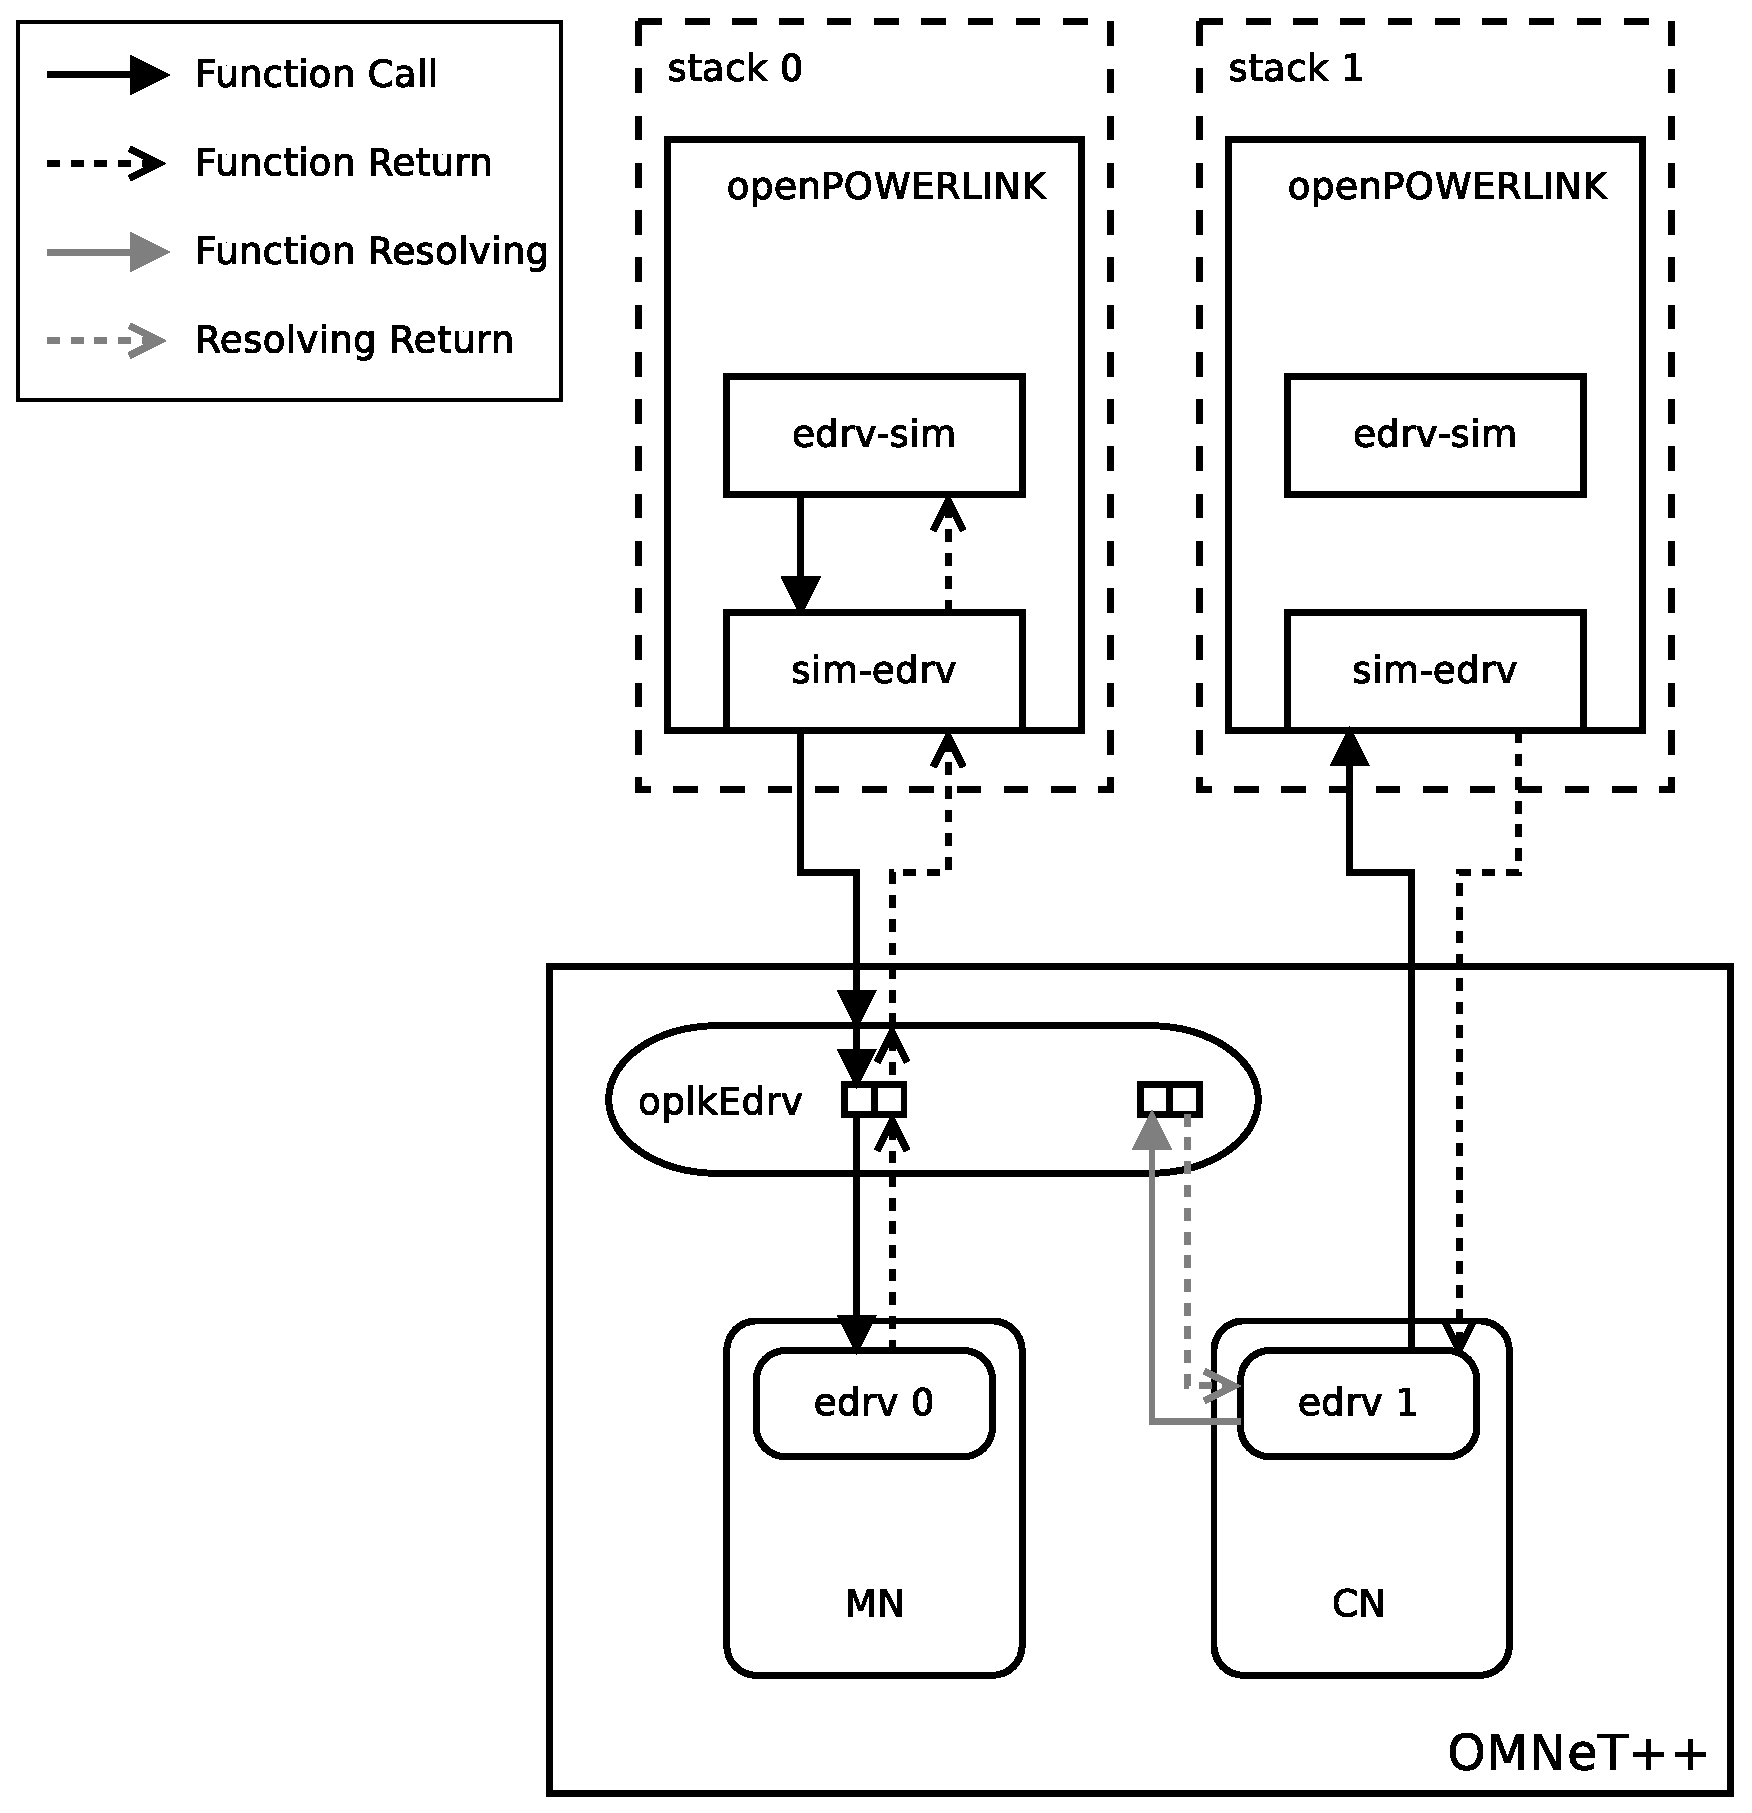
\includegraphics[width=0.7\linewidth]{simulation_instances}
    \caption{Hierarchical overview of the simulation environment, embedded modules the stack interface and simulation interface.}
    \label{fig:simulation_instances}
\end{figure}

The implementation of \emph{OplkBase}, \emph{SharedLibraryHelper} and \emph{OplkEdrv} are shown in appendix section \ref{app:simulation_stackif}.

The further implementation and structuring of the according OMNeT++ modules is described in the following section.

\subsection{Stack module}
\label{sec:porting_stack_stackmodule}

The previous mentioned OMNeT++ modules representing components within the openPOWERLINK stack and invoked by a derived class of \emph{OplkBase} are located in the \emph{stack} folder.
These modules provide the functions which implement the required functionalities for the openPOWERLINK stack.
The combination of these modules illustrate a single openPOWERLINK stack module and represent a single openPOWERLINK stack instance.

\begin{figure}
    \centering
    %TODO make screenshot and embedd
    %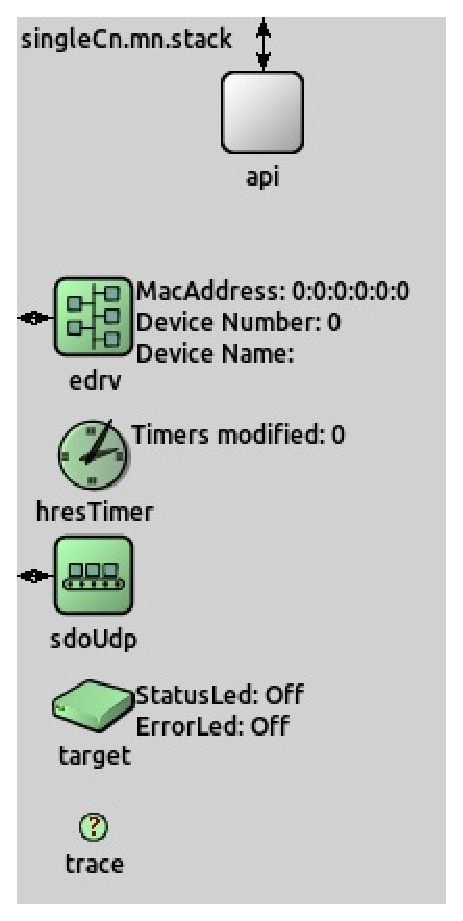
\includegraphics[width=0.7\linewidth]{simulation_stack_module}
    \caption{Composition of compound module representing the openPOWERLINK stack.}
    \label{fig:simulation_stack_module}
\end{figure}


\section{Simulated nodes}
\label{sec:porting_nodes}
%TODO explain different types of nodes

\subsection{Generic node}
\label{sec:porting_nodes_generic}
%TODO explain hierarchy and components of generic node with demo, app and event

\subsection{MN}
\label{sec:porting_nodes_mn}
%TODO explain special properties of MN

\subsection{CN}
\label{sec:porting_nodes_cn}
%TODO explain special properties of CN

%As described in section \ref{sec:oplk_platform} multiple modules contain platform specific functionalities.
%The openPOWERLINK stack can be built with various configurations, depending on the settings and the compositions configured individually more or less platform specific modules are used.
%These configurations are defined within the different projects in the \emph{proj} folder, as explained in section \ref{sec:oplk_structure_proj}.
%
%\section{Analyze of existing projects}
%\label{sec:porting_projects}
%
%\subsection{liboplkmn}
%\label{sec:porting_projects_liboplkmn}
%
%The \emph{liboplkmn} represents a \emph{MN} library consisting of a single library including the user and kernel space.
%Analyzing the \emph{liboplkmn} for linux results in following modules which must be ported:
%
%\begin{itemize}
%    \item Target
%    \item Timer
%    \item Edrv
%    \item \emph{SDO} via \emph{UDP}
%    \item Trace
%\end{itemize}
%
%The first step for the implementation of the \emph{MN} library for OMNeT++ is the integration in the configuration and build process within the openPOWERLINK stack.
%Therefore an according options file and toolchain file for integration in the \emph{CMAKE} process are created.

